\documentclass[letterpaper,fleqn]{article}
\usepackage[spanish,es-noshorthands]{babel}
\usepackage[utf8]{inputenc} 
\usepackage[papersize={6.5in,8.5in},left=1cm, right=1cm, top=1.5cm, bottom=1.7cm]{geometry}
\usepackage{mathexam}
\usepackage{amsmath}
\usepackage{graphicx}

\ExamClass{
\includegraphics[height=16pt]{Images/logo-sed.png} Cálculo $11^{\circ}$}
\ExamName{Nivelación 4 período}
\ExamHead{
\includegraphics[height=16pt]{Images/logo-colegio.png} IEDAB}
\newcommand{\LineaNombre}{%
\par
\vspace{\baselineskip}
Nombre:\hrulefill \; Curso: \underline{\hspace*{48pt}} \; Fecha: \underline{\hspace*{2.5cm}} \relax
\par}
\let\ds\displaystyle

\begin{document}
\ExamInstrBox{
Respuesta sin justificar mediante procedimiento no será tenida en cuenta en la calificación. Escriba sus respuestas en el espacio indicado. Tiene 45 minutos para contestar esta prueba.}
\LineaNombre
\begin{enumerate}
 \item Observe las gráficas de $f$ y $g$. Úselas para evaluar cada límite si existe. Si no existe, explique por qué.
\begin{center}
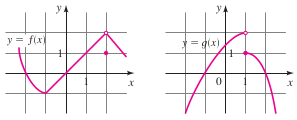
\includegraphics[scale=.8]{Images/funciones_fyg.png} 
\end{center}
\begin{enumerate}
\item $\ds{\lim_{x\rightarrow 2}}[f(x)+g(x)]$\noanswer
\item $\ds{\lim_{x\rightarrow 0}}[f(x)g(x)]$\noanswer
\item $\ds{\lim_{x\rightarrow -1}}\dfrac{f(x)}{g(x)}$\noanswer
\end{enumerate}
 \end{enumerate}

\end{document}
